\begin{appendices}
  \addtocontents{toc}{\protect\setcounter{tocdepth}{1}}
    \makeatletter
    \addtocontents{toc}{%
      \begingroup
      \let\protect\l@chapter\protect\l@section
      \let\protect\l@section\protect\l@subsection
    }
    \makeatother

    \chapter{User Manual}
      This document is also available online: \\ http://bit.ly/points\_extraction\_user\_manual

\noindent\hrulefill

\noindent This guide will list steps to complete the analysis for a single arbitrary discussion. The only software that you need to install on your computer is Docker and Docker Compose. Docker hosts lightweight virtual machines called containers that run each of our services.

\section{Installation}
\begin{enumerate}
	\item{\href{https://docs.docker.com/engine/installation/}{Install Docker} and the \href{https://docs.docker.com/compose/install/}{Docker Compose interface}. This varies depending on the host operating system.}
	\item{Check that you can run \texttt{docker ps} and see output starting: \texttt{CONTAINER ID...}}
	\item{Change directory into the project folder \texttt{cd {project-folder-path}}}
	\item{Run \texttt{docker-compose build}, this will download all the dependencies for each of the project's services. This includes a series of operating system images and the CoreNLP framework and will take some time (allow 20-25 mins on a 20mbps connection, time also depends on the resources allocated to Docker).}
\end{enumerate}

\section{Setting Up a Corpus}
\begin{enumerate}
	\item{First you need to get a corpus in place to run the analysis on. This guide will talk you through using the Abortion corpus we used. Download the corpus to the \texttt{analysis\_api} folder: \\  \texttt{curl -L http://bit.ly/1QxG9i7 > analysis\_api/abortion.zip}}
	\item{Now unzip the downloaded corpus: \\ \texttt{unzip analysis\_api/abortion.zip -d analysis\_api/abortion \&\& \\ mv analysis\_api/abortion/**/* analysis\_api/abortion/ \&\& \\ rm -r analysis\_api/abortion/5*}}
	\item{(OPTIONAL) Inspect a corpus file: \texttt{cat analysis\_api/abortion/post\_1}. Lines like \texttt{\#key=value} are parsed into metadata. These are optional.}
	\item{It is now time to start a console in the \texttt{analysis\_api} service. To do this run: \texttt{docker-compose run analysis\_api /bin/bash}.}
	\item{You will now have a new prompt \texttt{/app\#}. The current directory is \texttt{analysis\_api}, file changes are synced between this container and the host. Type \texttt{ls} and you will see the contents of the \texttt{analysis\_api} folder.}
	\item{Before extracting points from the corpus we need to clean the posts for invalid characters and parse any metadata. Run \texttt{ruby clean.rb abortion} to do this for all of the files in the raw abortion corpus we downloaded.}
\end{enumerate}

\section{Extracting Points}
\begin{enumerate}
	\item{You are now ready to extract a list of points from the corpus. To do this run \texttt{ruby collector.rb abortion}. This will take around 10-15 mins and is quite an intensive task. Output is written to \texttt{abortion\_points.txt} in the \texttt{analysis\_api} directory. This will be a large file (approx. 50mb), The first line is a list of topics and the following lines represent each point in JSON.}
	\item{When you have finished running the points extraction process you  can exit the analysis\_api console with \texttt{exit}.}
\end{enumerate}

\section{Cleaning/Curating Points}
\begin{enumerate}
	\item{To prepare the list of points for use in summarization they must first be reformatted. First you need to move your extracted points file into the \texttt{curator} directory. From the project root run: \\ \texttt{mv analysis\_api/abortion\_points.txt curator/abortion\_points.txt}}
	\item{From the project root directory run \texttt{docker-compose run curator /bin/bash} to get a console ready to run the curation task.}
	\item{To clean the list for summarization run: \\ \texttt{go run main.go abortion\_points.txt > abortion\_points\_clean.txt}}
\end{enumerate}

\section{Generating Summaries}
\begin{enumerate}
	\item{First get a clean list of points to use in generating the summary. From the project root run: \\ \texttt{mv curator/abortion\_points\_clean.txt summarizer/abortion\_points\_clean.txt}.}
	\item{Now run: \texttt{docker-compose run summarizer /bin/bash} to get a console prepared for generating summaries.}
	\item{To generate a summary for your clean list of points run: \texttt{ruby summarizer.rb abortion\_points\_clean.txt}}
	\item{This will save a file in the \texttt{summarizer} directory called \texttt{abortion\_formatted.html}. This is the end result and should be viewed in a browser.}
\end{enumerate}




    \chapter{Maintenance Manual\label{app:maintain}}
      This document is also available online at: \\ http://bit.ly/points\_extraction\_maintenance\_manual

\noindent\hrulefill

\noindent This document is intended to describe how the different components may
be adjusted in future work. Some features and potential adjustments are
described using references to key sections of code.

\section{Points Extraction}

Extracting points as part of generating a summary for a debate is
described in the user manual. This however makes use of the
\texttt{analysis\_api} to collect points. This should could be seen as
an example of how one might use the \texttt{points\_api} service. This
section of code in the \texttt{collector.rb} file in the
\texttt{analysis\_api} folder is where points for text are extracted.

\begin{minted}[breaklines=true]{Ruby}
# specify where the points_api is running
uri = URI('http://points_api:4567/')
# create an http client to make the upcoming requests
http = Net::HTTP.new(uri.host, uri.port)
# for each of the posts in the discussion corpus, extract the points.
posts.each_with_index do |post, index|
  # prepare a request object
  # [post text, topics of interest and required point attribute keys]
  query = { text: post["content"], topics: topics, keys: %w(string pattern) }.to_json
  # make the request against the points api
  req = Net::HTTP::Post.new(uri)
  req.body = query
  # parse the response from the points api
  data = JSON.parse(http.request(req).body)
  # write each point in the response to the points file
  data.map { |p| out_file.write("#{p.merge(post).to_json},\n") }
end
\end{minted}

This shows that extracting points with the points api is a simple
request/response process. This excerpt from the points\_api shows in
part how requests for points are handled. The input text is split into
sentences (each with a dependency parse) and these are saved in turn to
the neo4j database.

\begin{minted}[breaklines=true]{Ruby}
# save each group of sentences
sentences.each_slice(5).each do |group|
    # Generate a Cypher query and execute it to save them all to the database
    query_string = neo4j_client.generate_create_query_for_sentences(group)
    neo4j_client.execute(query_string)
end
# find all the verbs that match one or more of their frames.
matches = PointsExtraction.matches_for_verbs(neo4j_client, frames, frame_queries)
# upgrade matches to points with extracts, collect points.
points += PointsExtraction.points_for_matches(neo4j_client, matches, data['topics'], data['keys'])
\end{minted}

\section{Summary Customization}

It is also likely that the summary content will need to be adjusted. The
key files used in generating summaries are \texttt{summary.rb} and
\texttt{template\_formatted.html.erb} in the summarizer folder.

Summaries are generated by calling \texttt{build}. This section below
shows how this method generates each section of the summary in turn.
Removing one of these lines will stop that section from being generated.

\begin{minted}[breaklines=true]{Ruby}
@counter_points = generate_counter_points; print "."
@related_points = generate_related_points; print "."
@negated_points = generate_negated_points; print "."
@common_points = generate_common_points; print "."
@longer_points = generate_longer_points; print "."
@commonly_discussed_topic_points = generate_commonly_discussed_topic_points; print "."
@multiple_topic_points = generate_multiple_topic_points; print "."
@question_points = generate_question_points; print ".\n"
\end{minted}

If a section is removed it must also be removed from the summary
template. Sections in the template look like this and should be removed
if the summary content has been adjusted.

\begin{minted}[breaklines=true]{XML+RUBY}
<p>Points about <strong>multiple topics</strong>:</p>
<% @summary.multiple_topic_points.each do |point| %>
  <blockquote>
    <p><%= Presenter.format(point["String"], @summary.topics) %></p>
  </blockquote>
<% end %>
\end{minted}

Summaries can also be customised in other ways. When initializing a
summary with
\texttt{Summary.new(title,\ points,\ topics,\ point\_count)} we can see
that a title (`abortion'), list of points, topics, and a point\_count is
required. Increasing the \texttt{point\_count} will create longer
summaries.

\section{Project Source Listing}

This section lists all top level files and folders as well as sub folders containing source code. Some files are omitted in the interest of brevity.

\subsection*{analysis\_api}
  This service makes used of the points api to collect a list of points for an entire discussion.
  \begin{itemize}
    \item
      \texttt{Dockerfile}: This is a file that contains the specification for an container to be used in collecting points for a corpus. This is used by Docker Compose to build the container image. It is built on the base Ruby docker image.
    \item
      \texttt{clean.rb}: This is a script for cleaning a corpus of posts. The key line: \texttt{content.chars.select(\&:valid\_encoding?).join} forcibly removed invalid characters. This file also parses post metadata lines (\#key=value) and saves the input files as JSON.
    \item
      \texttt{collector.rb}: This should be seen as a client for the points\_api. This script iterates the post files in the specified corpus directory and uses the points\_api to collect points for each post in turn.
  \end{itemize}

\subsection*{corenlp\_server}
  This is a shell representing CoreNLP image as used as a service by other components.
  \begin{itemize}
    \item
      \texttt{Dockerfile}: This is a more complex, custom Dockerfile for the CoreNLP service. Used via docker-compose and based on the Java base image this file specifies how the CoreNLP server environment should be configured for use by other services.
  \end{itemize}

\subsection*{curator}
  This single program service implements points curation.
  \begin{itemize}
    \item
      \texttt{Dockerfile}: This simple docker file specifies a Golang environment to run the points curation task.
    \item
      \texttt{main.go}: This is file implements the entirety of the points curation task. It's process is described in detail in \ref{chap:point-curation}.
  \end{itemize}

\subsection*{docker-compose.yml}
  This file is used as the basis for docker-compose in the project. The contents represent all local provisioning settings for services and how they are connected to one and other in YAML syntax. For example, we can see that the analysis\_api is connected with \texttt{links:} to the points and topic API --- as diagrammed in Chapter \ref{chap:system-architecture}. This file also specifies the locations of all Dockerfiles for each service in the project.

\subsection*{docs}
  This folder contains the project's documentation source.
  \begin{itemize}
    \item
      \texttt{presentation}: This folder contains the slides used in presenting the tool for at the social media workshop in Study 3.
    \item
      \texttt{report}: This folder contains all files used to generate the project report.
  \end{itemize}

\subsection*{evaluation}
  This folder contains all resources used or generated as part of the evaluation.
  \begin{itemize}
    \item
      \texttt{evaluation\_sheet}: This folder contains the evaluation forms used in Study 3.
    \item
      \texttt{extract\_comparison\ (RESULTS)}: This folder contains the results from Study 2 in CSV format as exported from Amazon Mechanical turk.
    \item
      \texttt{summary\_comparison\ (RESULTS)}: This folder contains the results from Study 1 in CSV format as exported from Amazon Mechanical turk.
    \item
      \texttt{extract\_ranking.rb}: This is a script that contains the same bigram ranking code used in generating summaries. It can be used to get scores for a group of extracts.
    \item
      \texttt{process\_extract\_comparison.rb}: This is a general purpose script to process the results from Study 2. It prints the results in a variety of formats.
    \item
      \texttt{process\_summary\_comparison.rb}: This is a general purpose script to process the results from Study 1. It prints the results in a variety of formats.
    \item
      \texttt{r\_analysis/}: This folder contains the r script files used to generate the graphs and significance figures used in the results section.
    \item
      \texttt{study3\_comments.txt}: This file contains the typed comments from the Study 3 participants.
    \item
      \texttt{survey/}: This folder contains a series of files that were used to generated the questionnaires for Studies 1 \& 2. These process summaries as exported by the summarizer into HTML that is read for use on Mechanical Turk's HIT interface.
  \end{itemize}

\subsection*{points\_api}
  This is the core system service and is largely reusable. It is implemented as a simple web service that, for a request containing text, returns the results of points extraction analysis.
  \begin{itemize}
    \item
      \texttt{Dockerfile}: This defines the configuration required to run an instance of the points API. This includes installing the dependencies from the Gemfile.
    \item
      \texttt{Gemfile}: The Gemfile lists the requirements for this service. The points api is implemented as a basic Sinatra application and makes used of the Sinatra microframework. It also requires an XML parser (nokogiri) and the ruby neo4j wrapper.
    \item
      \texttt{app.rb}: This file implements the core of the points extraction service. It defines a root route that that accepts requests for points analysis. It splits the text into chunks and extracts sentences before triggering the points analysis.
    \item
      \texttt{frame\_queries}: This folder contains all the frame queries in Cypher for each of the frame patterns (\texttt{NP VERB NP} etc.). The folder also contains variations of queries for copula verbs and the generic frame query.
    \item
      \texttt{groups.json}: This is a JSON representation of the VerbNet database. It is not only used for inspecting verb classes when debugging.
    \item
      \texttt{lib}:

      \begin{itemize}
        \item
          \texttt{corenlp\_client.rb}: This is a wrapper used in requesting dependency parse information from the CoreNLP service.
        \item
          \texttt{frame.rb}: This class represents a frame. Frames loads from the index are used to initialize instances of this class. This exposes a number of helper methods used in processing frames and points.
        \item
          \texttt{neo4j\_client.rb}: This is a wrapper for the Neo4j services and is used to execute queries and fetch results using a simplified interface.
        \item
          \texttt{node.rb}: This class extends the Neo4j::ActiveNode class and defines the structure that should be used to save tokens in the Neo4j database. This includes attributes and dependency relations to other nodes.
        \item
          \texttt{points\_extraction.rb}: This is the central file to extracting points from text. This is called from the application twice, first to get the verbs that have valid frame matches from in the database and then, for each of these, to get the extract information for the match as a complete point, ready to send in the response.
        \item
          \texttt{relation.rb}: This class extends the Neo4j::ActiveRel class and defines the structure of a dependency graph edge. These objects only have a single label attribute and connect two tokens nodes in the graphs.
        \item
          \texttt{utils.rb}: This implements a series of helper functions used in the extraction  of points.
      \end{itemize}
    \item
      \texttt{tasks}:

      \begin{itemize}
        \item
          \texttt{parse\_verb\_net.rb}: This is a script used in parsing the XML information from VerbNet. VerbNet is not stored in it's original form in the project source but is available for download here: \\ http://verbs.colorado.edu/verb-index/vn/verbnet-3.2.tar.gz
      \end{itemize}
    \item
      \texttt{verbs.json}: This is the verb index. It is loaded by the application and used to lookup frame each verb found in the input text.
  \end{itemize}

\subsection*{stock\_summarizers}
  This folder contains other summarizer implementations used in evaluation.
  \begin{itemize}
    \item
      \texttt{summarizer\_topic.py}: This is the implementation of the `Stock' summarizer used in the evaluation that was adjusted to run as part of the summary generation process. Originally sourced from \\ http://homepages.abdn.ac.uk/advaith/pages/teaching/NLP/practicals/Practical3.zip
  \end{itemize}

\subsection*{summarizer}
  This folder contains files for the summarizer service, the service that processes a list of extracted points into HTML summaries.

  \begin{itemize}
    \item
      \texttt{Dockerfile}: This defines the Ruby image required to run the summarization task. As part of the build process the requirements from the Gemfile are installed.
    \item
      \texttt{Gemfile}: This lists the requirements for the summarizer service. This service makes use of \texttt{differ} --- a string diffing library --- and \texttt{levenshtein} a library for calculating the Levenshtein distance of two strings. The debugger Pry is also required when debugging the service.
    \item
      \texttt{antonyms.json}: This is a key value index of all antonyms used in the counter point analysis. This is sourced from the Wordnet NLTK corpus. Each word is a key, each value is a list of its antonyms.
    \item
      \texttt{condense.rb}: This module implements a means of merging strings that are similar. Making use of the differ gem, this can take a pair of strings e.g. \blockquote{\textit{Abortion is not a right}} and \blockquote{\textit{Abortion is a right}} and output: \blockquote{\textit{Abortion is \textbf{\{}not\textbf{\}} a right}}.
    \item
      \texttt{counters.rb}: This file implements the search process for both counter and negated points.
    \item
      \texttt{curator.rb}: This implements the selection of the best extract for a list of points. This was tested in Study 2. \texttt{select\_best}, given a list of points, will return the highest scoring one from the bigram model.
    \item
      \texttt{paragraphizer.rb}: This file is was used in the generation of the Plain summary style for the evaluation. It is not used in the current summarizer implementation to keep the basic analysis process as simple as possible.
    \item
      \texttt{presenter.rb}: This module implements the clean and format methods. Given a string such as \blockquote{\textit{, abortion is a right - }} it will output \blockquote{\textit{Abortion is a right.}}. Every extract is cleaned using the methods defined here before being included as part of a summary.
    \item
      \texttt{related.rb}: This module implements the identification of related points.
    \item
      \texttt{summarizer.rb}: This script brings all the other modules in this service together and uses them to analyze points and produce a summary from them.
    \item
      \texttt{summary.rb}: This class implements the summary object. The summarizer uses an instance of this class to build a summary before passing it to an ERB template and writing an HTML summary to disk.
    \item
      \texttt{template\_formatted.html.erb}: This is the template used specify the format a summary object should take when presented in HTML. Given a summary object this fills a series of sections to complete the summary using the information stored in the summary.
    \item
      \texttt{utils.rb}: This file contains a utility function for collecting a key value representation of the duplicates in a list. This is used in the summary class.
  \end{itemize}

\subsection*{topic\_api}
  This folder contains the files that represent the topic api, a service that wraps the third-party LDA topic modeler.
  \begin{itemize}
    \item
      \texttt{Dockerfile}: This defines the docker image used to run an instance of the topic api. This sets up a base Ruby installation and installs the project gem dependencies.
    \item
      \texttt{Gemfile}: This lists the three service dependencies. Similar to the points api, this service is also implemented as a Sinatra application. It also requires a Ruby wrapper to a C LDA (Latent Dirichlet allocation) implementation and the Pry debugger.
    \item
      \texttt{app.rb}: This file implements the topic api service. It exposes a route that can accept requests containing a body of text. From this is runs the LDA analysis and returns the topic words as a response.
  \end{itemize}

\subsection*{utilities}
  This folder contained other experimental implementations. Currently it only includes the graph representation plotter.

  \begin{itemize}
    \item
      \texttt{plotter}:

      \begin{itemize}
      \item
        \texttt{graph.html}: This is a template, standalone template for the graph representation of points as seen in Appendix \ref{app:disc_graph}.
      \item
        \texttt{plot.rb}: This script takes a list of point patterns and uses the graph HTML template to build a resulting HTML file.
      \end{itemize}
  \end{itemize}


    \chapter{Discussion Graph Representation\label{app:disc_graph}}
      \begin{figure}[h]
        \centering
        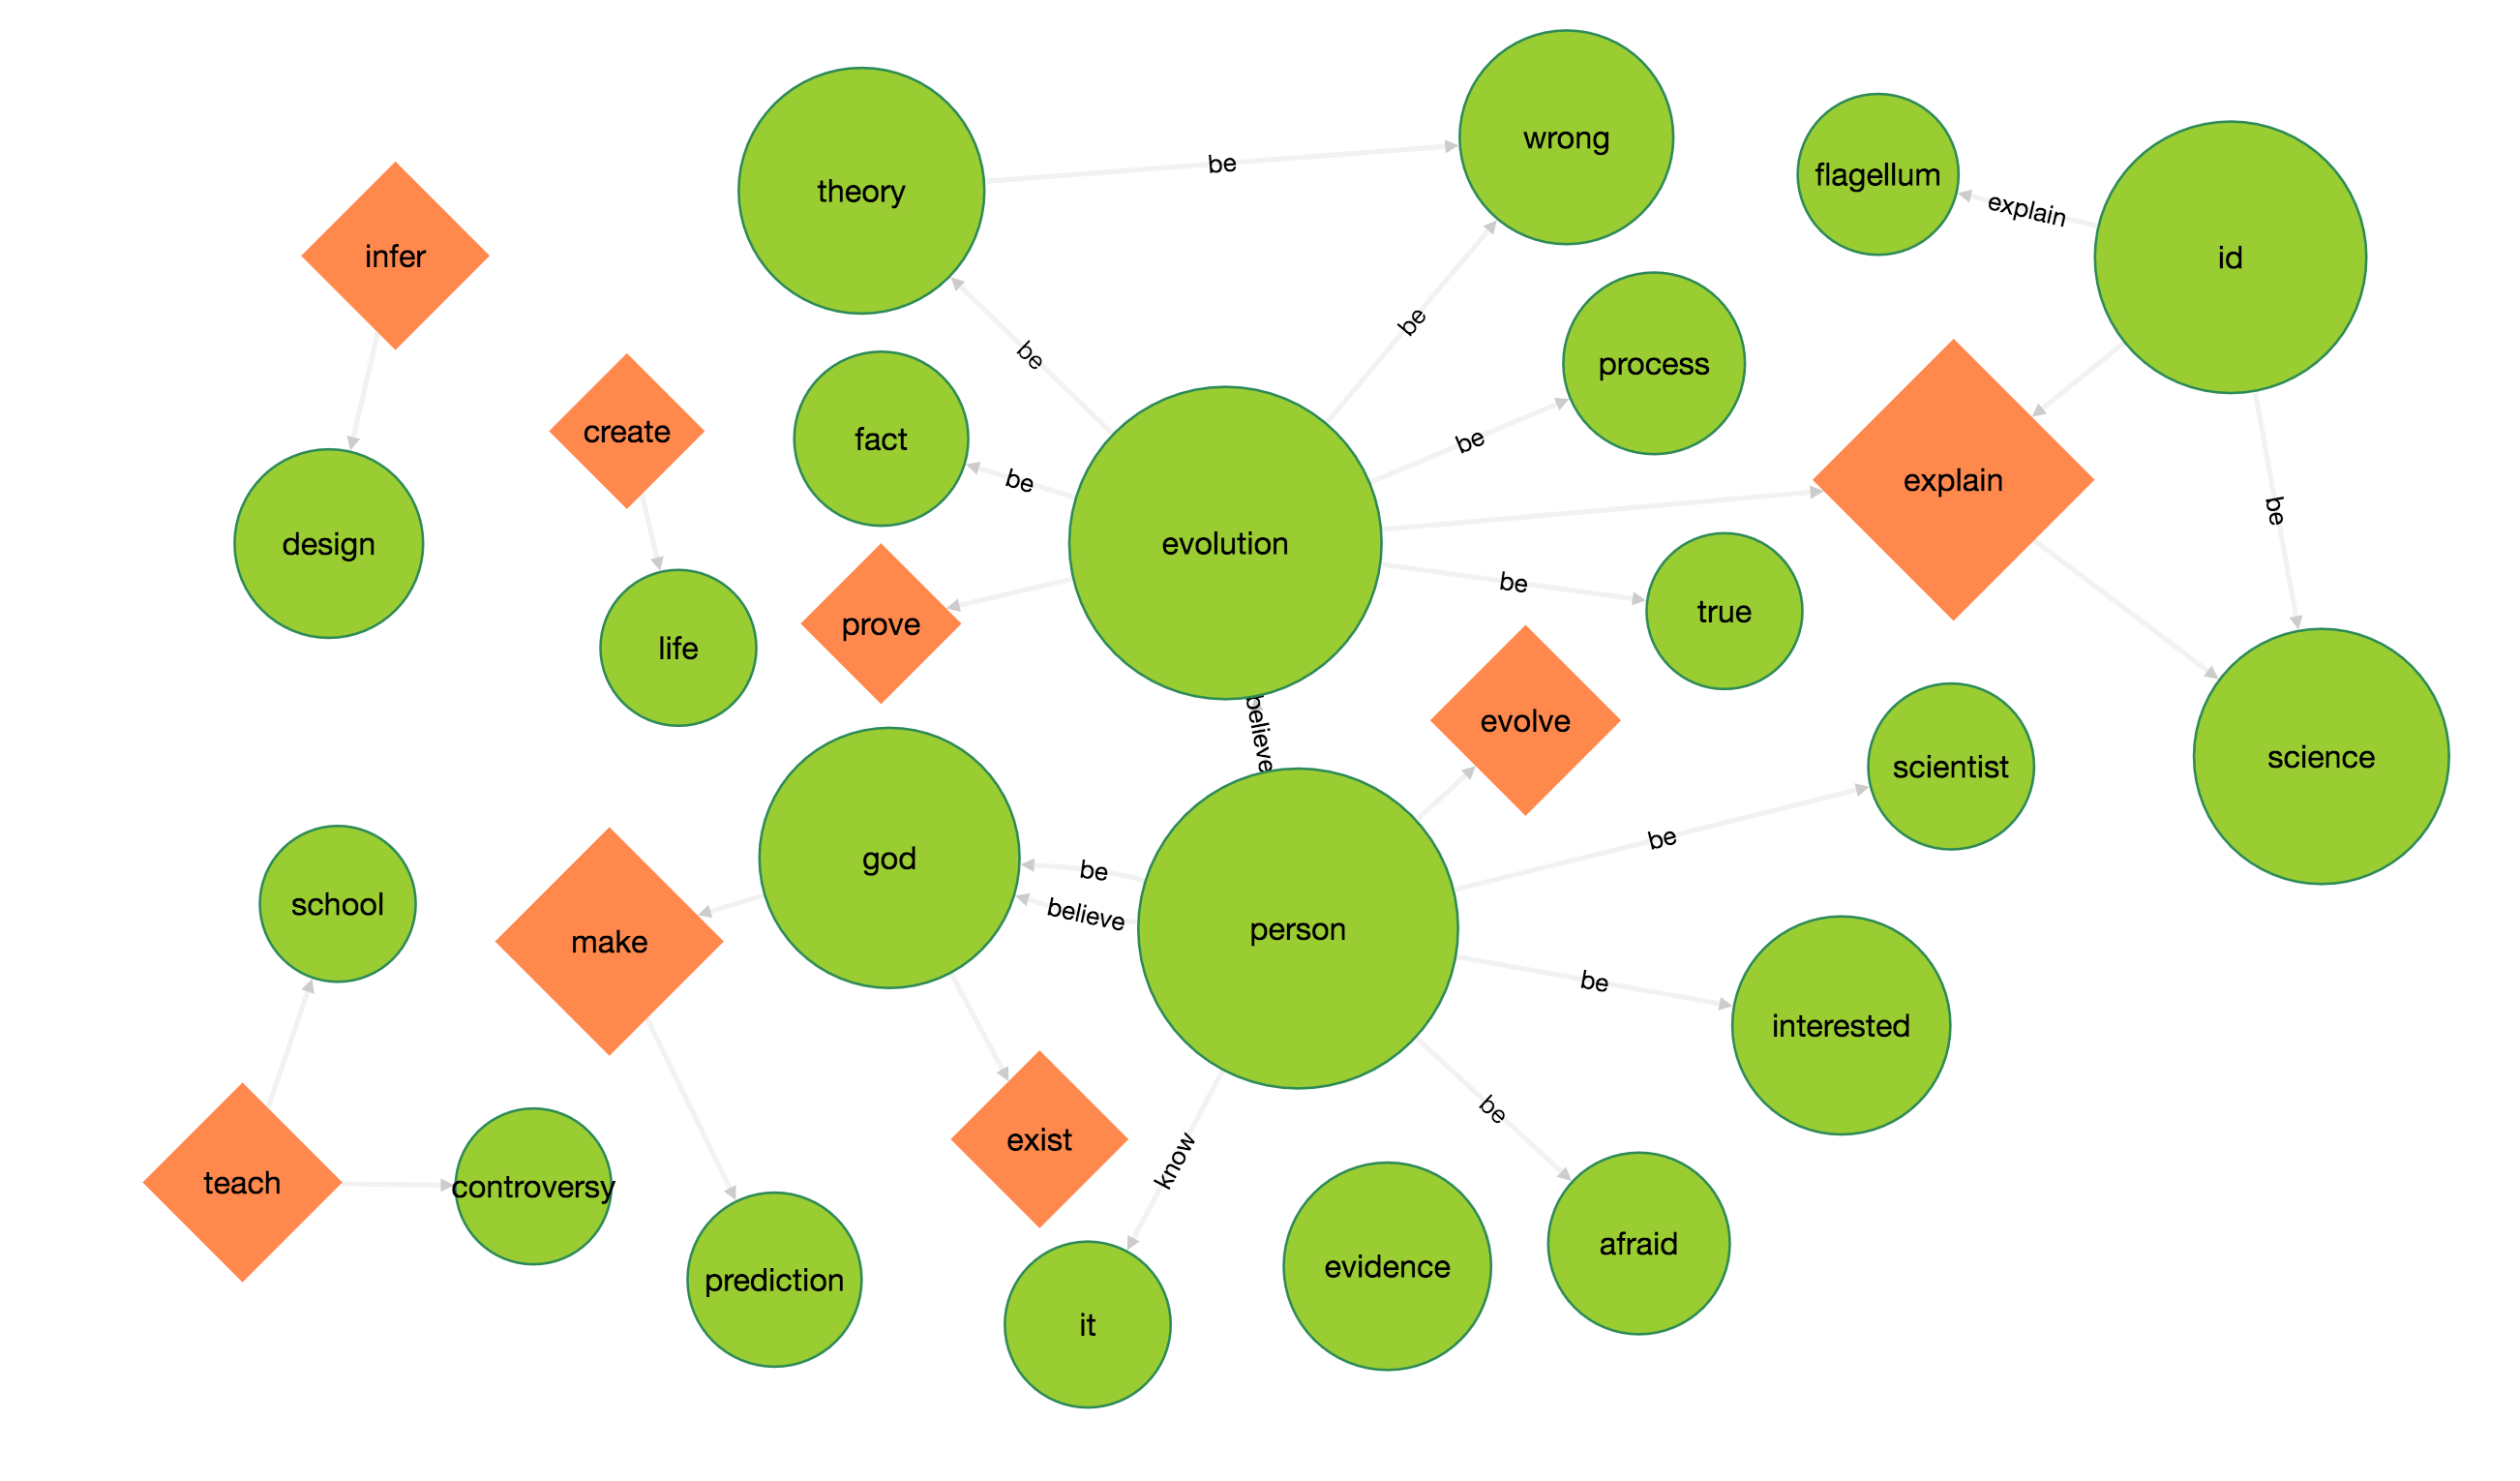
\includegraphics[width=0.8\textwidth]{disc_graph}
        \caption{A sample graph representation of the abortion discussion}
      \end{figure}

    \chapter{Blacklists\label{app:blacklists}}
      \section{Ambiguous subjects}
        \textit{it, that, this, which, what}

      \section{Disallowed Person Actions}
        The following verbs are not allowed in a 2 component point with a \texttt{PERSON.nsubj}:

        \textit{agree, argue, ask, begin, believe, believe, call, care, change, close, come, come, continue, debate, disagree, end, explain, fail, feel, feel, find, follow, get, go, go, guess, happen, hear, leave, live, lose, make, move, object, open, read, realize, refer, show, sit, speak, stand, start, support, take, talk, tell, think, try, understand, wonder, write}

      \section{Disallowed Points}
        \texttt{PERSON.nsubj be.verb} cannot be completed by: \textit{able, aware, correct, false, favor, glad, good, here, interested, likely, one, right, say, sorry, sure, true, willing, wrong}

        \noindent\texttt{PERSON.nsubj want.verb} cannot be completed by: \textit{have, what, what do}

        \noindent\texttt{PERSON.nsubj} cannot be completed by: \textit{say.verb what.dobj, mean.verb what.dobj, know.verb what.dobj, believe.verb what.dobj, see.verb what.dobj, see.verb argument.dobj, have.verb problem.dobj, tell.verb they.dobj, think.verb what.dobj, argue.verb in.prep fact.dobj, argue.verb with.prep you.dobj}

        \begin{itemize}
		  \item{debate.nsubj be.verb about.dobj}
		  \item{question.nsubj be.verb}
		  \item{make.verb claim.dobj}
		  \item{ask.verb yourself.dobj}
		  \item{thing.nsubj happen.verb}
		  \item{something.nsubj happen.verb}
        \end{itemize}

    \chapter{Evaluation Questionnaire Structure \label{app:evaluation-questionnaire-layouts}}
      \TBox[fill=red!15]{13cm}{
        \large Study 1 Questionnaire ($\times$6 variations in Latin Square) \\
        \normalsize
        \TBox[fill=black!1]{12.7cm}{
          \textbf{Section 1} Plain vs. Stock (see Appendix \ref{app:survey-section}) \\
          \small Order switches (3$\times$ Plain/Stock, 3$\times$ Stock/Plain)
          \normalsize

          \TBox[fill=white]{6cm}{
            Plain Summary (Topic A)
          }
          \TBox[fill=white]{6cm}{
            Stock Summary (Topic A)
          }
          \TBoxDash[fill=black!15]{12.4cm}{
            \textit{4 factor ratings; overall rating \& free text comment}
          }
        }
        \TBox[fill=black!1]{12.7cm}{
          \textbf{Section 2} Layout vs. Stock \\
          \small Order switches (3$\times$ Layout/Stock, 3$\times$ Stock/Layout)
          \normalsize

          \TBox[fill=white]{6cm}{
            Layout Summary (Topic \textbf{B})
          }
          \TBox[fill=white]{6cm}{
            Stock Summary (Topic \textbf{B})
          }
          \TBoxDash[fill=black!15]{12.4cm}{
            \textit{4 factor ratings; overall rating \& free text comment}
          }
        }
        \TBox[fill=black!1]{12.7cm}{
          \textbf{Section 3} Layout vs. Formatted \\
          \small Order switches (3$\times$ Layout/Formatted, 3$\times$ Form./Lay.)

          \small Summaries share content, only differ in formatting

          \small Layout summary reused from Section 2
          \normalsize

          \TBox[fill=white]{6cm}{
            Layout Summary (Topic \textbf{B})
          }
          \TBox[fill=white]{6cm}{
            Formatted Summ. (Topic \textbf{B})
          }
          \TBoxDash[fill=black!15]{12.4cm}{
            \textit{Overall rating only \& free text comment}
          }
        }
      }

      \vspace{2mm}
      \noindent\TBox[fill=green!15]{13cm}{
        \large Study 2 Questionnaire ($\times$6 variations) \\
        \normalsize
        \TBox[fill=black!1]{12.7cm}{
          \textbf{Section 1} Rating Extracts \\
          \normalsize

          \TBox[fill=white]{12.4cm}{
            Extract Set (Topic A) \textbf{($\times$3)} (see Appendix \ref{app:extract-survey-section})\\
            \TBoxDash[fill=black!15]{12.1cm}{
              \textit{Rating 1/5 per extract (approx. 10 extracts)}
            }
          }
        }
        \TBox[fill=black!1]{12.7cm}{
          \textbf{Section 2} Bigram vs. Random \\

          \TBox[fill=white]{6cm}{
            Bigram Summary (Topic A)
          }
          \TBox[fill=white]{6cm}{
            Random Summary (Topic A)
          }
          \TBoxDash[fill=black!15]{12.4cm}{
            \textit{Overall rating only \& free text comment}
          }
        }
      }

      \vspace{2mm}
      \noindent\TBox[fill=blue!15]{13cm}{
        \large Study 3 Questionnaire ($\times$2 variations each, $\times$6 variations total) \\
        \normalsize
        Participants had \textbf{two sheets}, each with different topics.
        \TBox[fill=black!1]{12.7cm}{
          \textbf{Section 1} Layout vs. Stock \\

          \TBox[fill=white]{6cm}{
            Layout Summary (Topic A)
          }
          \TBox[fill=white]{6cm}{
            Stock Summary (Topic A)
          }
          \TBoxDash[fill=black!15]{12.4cm}{
            \textit{Free text comments only}
          }
        }
      }

    \chapter{Summary Comparison Survey Section\label{app:survey-section}}
      \begin{figure}[h]
        \caption{An example study 1 survey section comparing a plain and stock survey.}
        \centering
        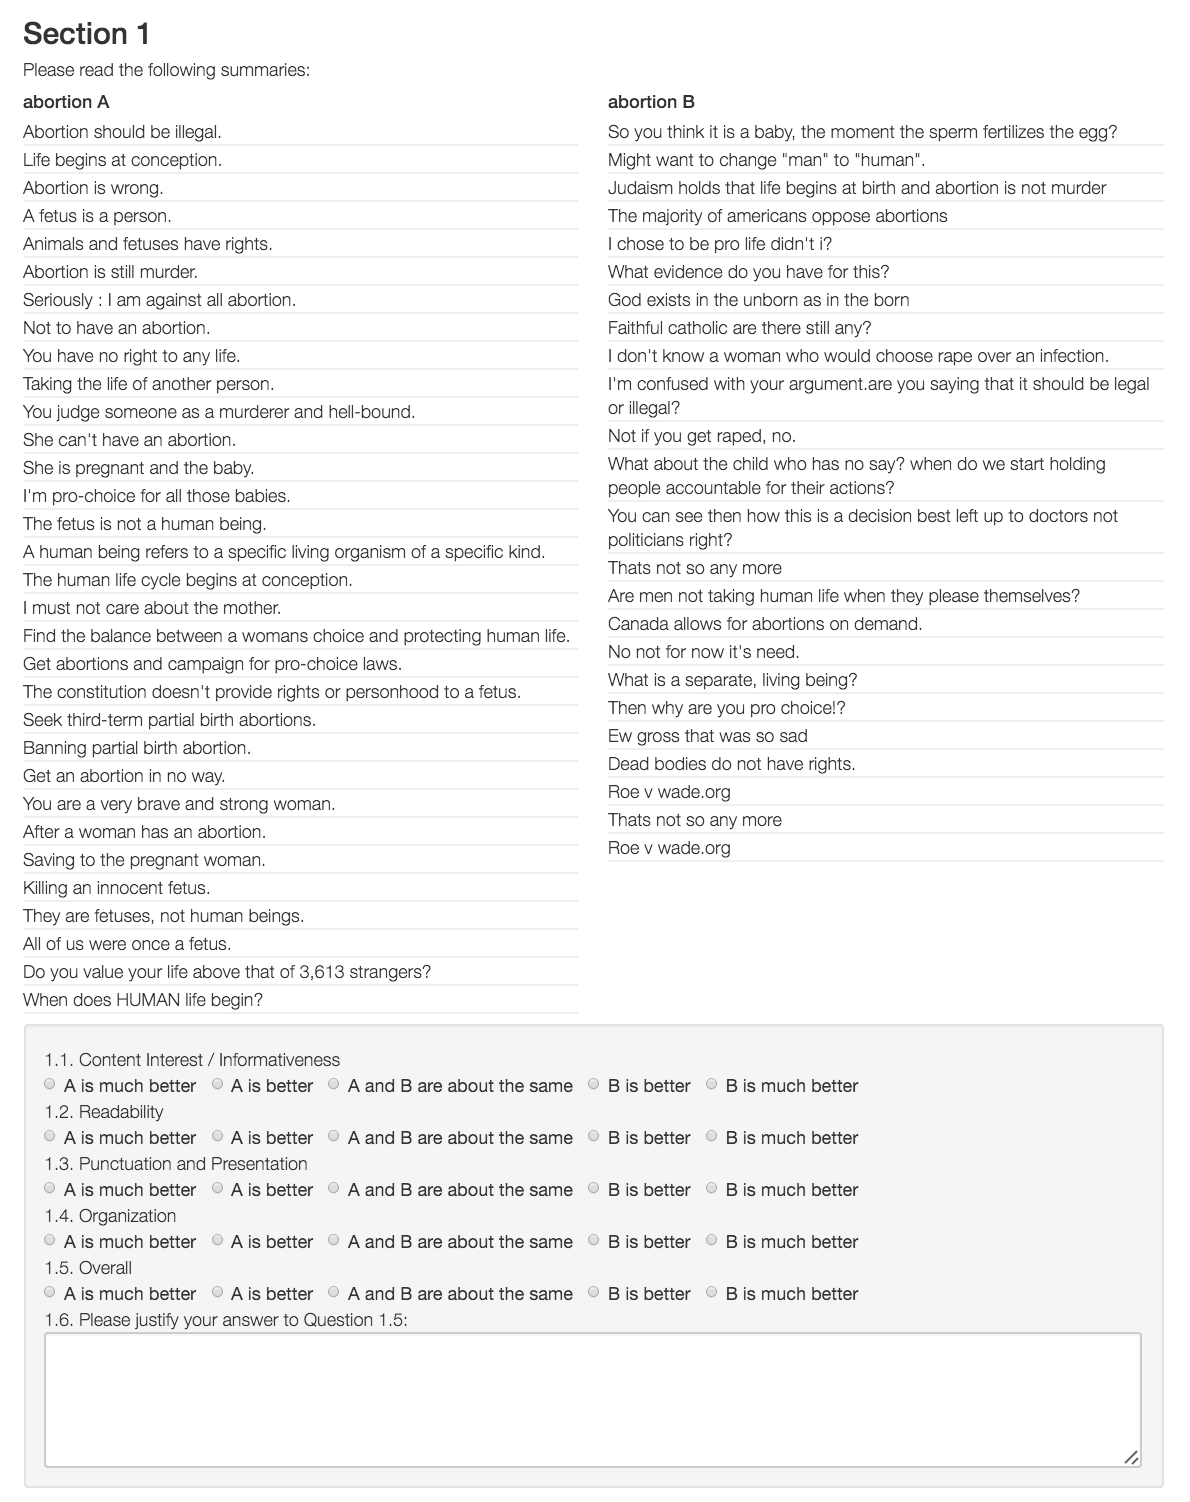
\includegraphics[width=0.9\textwidth]{survey}
      \end{figure}

    \chapter{Extract Survey Section\label{app:extract-survey-section}}
      \begin{figure}[h]
        \caption{An example study 2 survey section where participants rated extracts.}
        \centering
        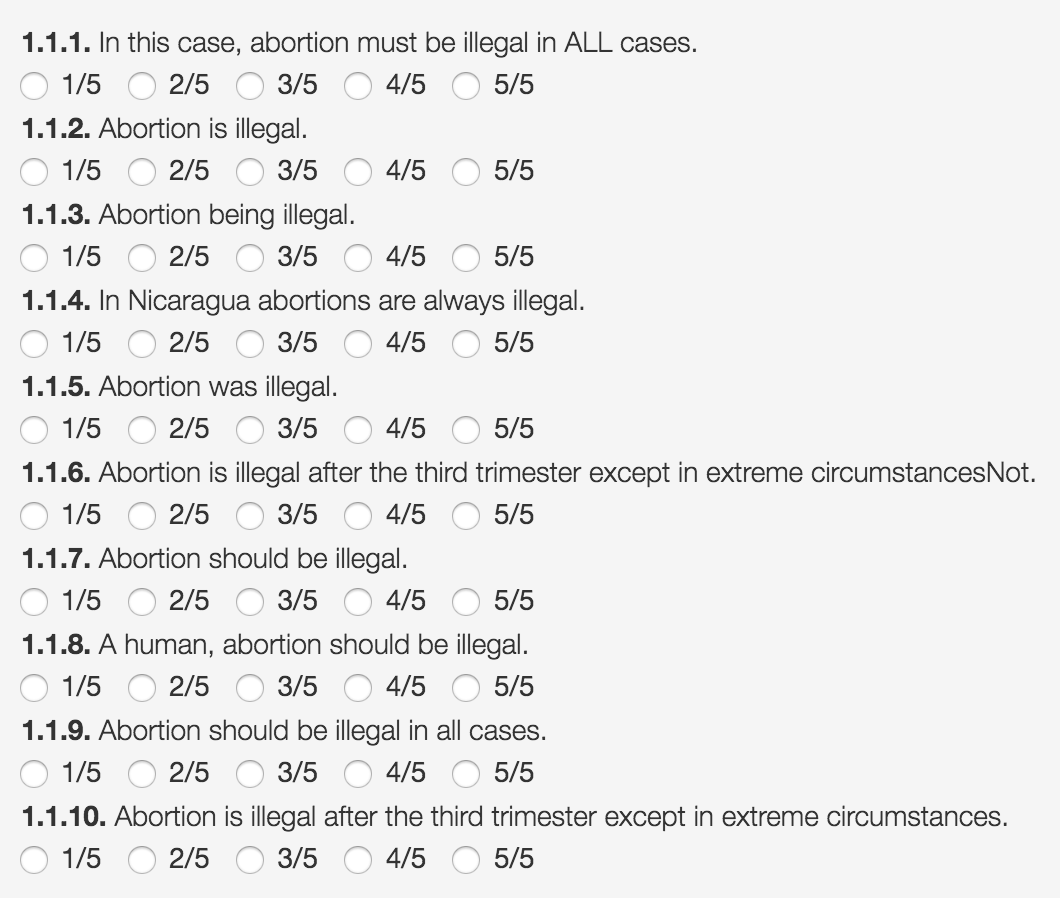
\includegraphics[width=0.9\textwidth]{survey2}
      \end{figure}

  \addtocontents{toc}{\endgroup}
\end{appendices}
